\begin{figure}[h]
    \centering
    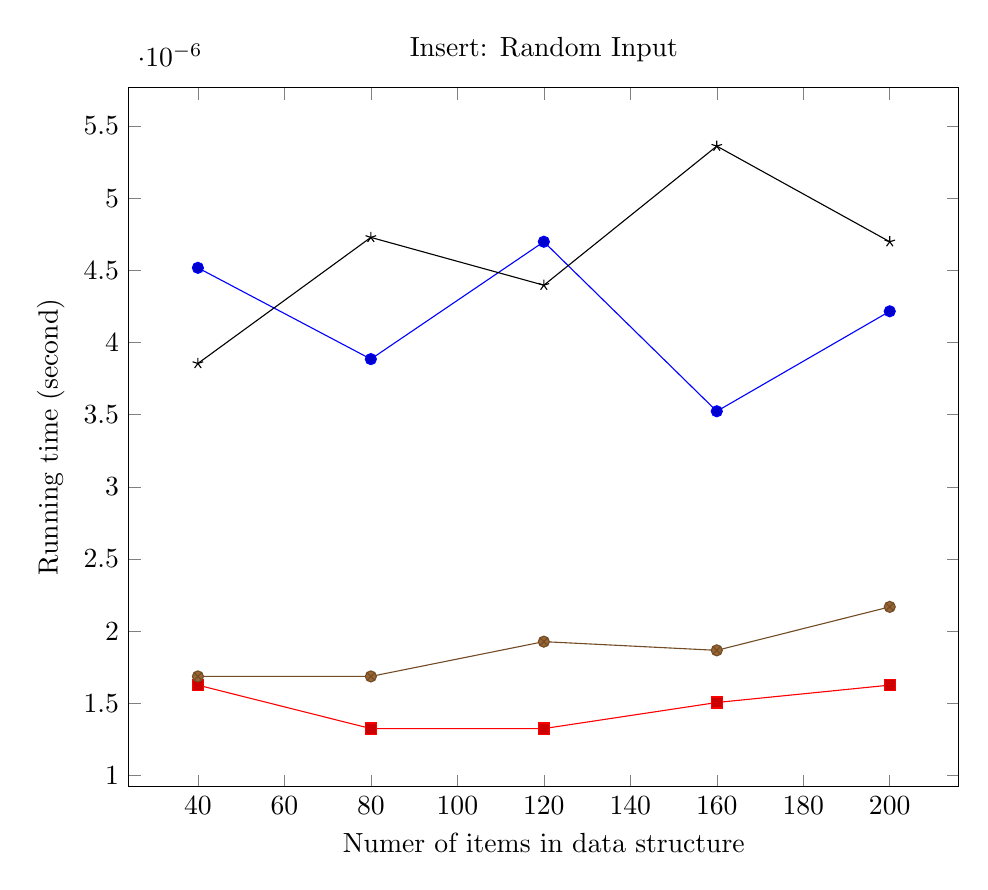
\begin{tikzpicture}
        \begin{axis}[
            xlabel={Numer of items in data structure},
            ylabel={Running time (second)},
            title={Insert: Random Input},
            width=\textwidth
        ]
		\addplot coordinates {
			(40, 4.517630051275104e-06)
			(80, 3.885161844096457e-06)
			(120, 4.698335253325997e-06)
			(160, 3.523751439994324e-06)
			(200, 4.2164547145236155e-06)
		};
		\addplot coordinates {
			(40, 1.626346818459079e-06)
			(80, 1.3251714817075904e-06)
			(120, 1.3251714817072435e-06)
			(160, 1.5058766837584836e-06)
			(200, 1.626346818459079e-06)
		};
		\addplot coordinates {
			(40, 1.6865818858093767e-06)
			(80, 1.6865818858093767e-06)
			(120, 1.9275221552105675e-06)
			(160, 1.8672870878606168e-06)
			(200, 2.1684624246121055e-06)
		};
		\addplot coordinates {
			(40, 3.855044310421829e-06)
			(80, 4.728452787001319e-06)
			(120, 4.397159916574856e-06)
			(160, 5.3609209941803125e-06)
			(200, 4.698335253325997e-06)
		};
        \legend{}
        \end{axis}
    \end{tikzpicture}
    \caption{Average of 0 operations, benchmarked every 0, starting at 0.}
\end{figure}